% !TeX spellcheck = en_UK
% ------------------------------------------------------
% RCGI: Research Centre for Gas Innovation 
% Latex Template
% please do not change documentclass options
% ---------------------------------------
\documentclass[11pt,a4paper]{report}

\usepackage{RCGIreport}

% use a preamble file if you want to insert additional packages
%
%\usepackage{algorithm}
%
\newcommand{\Rey}{\ensuremath{\mathrm{Re}}}




% see instructions below
\title{Project~00 -- \LaTeX\ Template for RCGI reports}
\doctype{\LaTeX\ Template for Scientific Report}
\docID{RCGI-AAA-BBB-CCC-DDD-EE}
\programme{CO$_2$ Abatement}
\projectnumber{00}

% Author lists
\author{Rafael S.\  Gioria\\ Annoyed with MS-WORD \\ \LaTeX\ Shall solve \\ author4 \\ author5\\ author6}
% Second column of authors in project
\authortwo{\it creator\\ fact \\ Solution\\ MSc \\ Post Doc \\ MSc }

% -- above commands
% \title{ } report title - Suggested: Project ## - name of the project
% \projectnumber{08} -- 1 or 2 digits
% \doctype{ } Doc types choices- Monthly Technical Report, Partial Technical Report, Final Technical Report, Partial Scientific Report, Final Scientific Report
% \programme{ ]  -- see options below - 3rd column assoiated with AAA 
%% \docID{ }  -- see long text below
%% RCGI	RCGI
%%
%% Identifies the Programme or area within the RCGI
%% AAA 	ENG    Engineering                     
%%    	PCH    Physical-Chemistry              
%%    	EEP    Economics & Energy Policies     
%%    	CAB    CO2 Abatement                   
%%    	KDF    Knowledge Diffusion             
%%    	TCT    Technology Transfer             
%%    	COM	   Communication	
%%
%% ## are the two digits of project number. Always use two digits, p.e. P04, P21, etc.
%% BBB		P##
%%
%% CCC		PSR		Partial Scientific Report 
%%  		FSR		Final Scientific Report   
%%		   	
%% DDD		###		Identifies the document number. Always use three digits.
%%
%% EE		##		Identifies the revision number. Always use two digits. Please use 00 for the original document.



\begin{document}

% -----------------------------------------
% CREATE coverpage - defined in RCGIreport.sty
\makecoverpage
% -----------------------------------------

% -----------------------------------------
% CREATE revision sheet
% -----------------------------------------
% EDIT HERE YOUR  list your revisions in the following format
% - each revision is a 4-tuple
% - separate each revision with comma ,
%{rev}{description}{app}{date},
%{rev1}{description1}{ap1p}{date1}
\revision{
{00}{initial commit}{RSG}{05/07/2020},
{01}{1st altered}{RSG}{07/07/2020},
{~}{~}{~}{~},
{~}{~}{~}{~},
{~}{~}{~}{~},
{~}{~}{~}{~}
}
% -----------------------------------------



% CREATE Table of Contents - do not change
\tableofcontents



% -----------------------------------------
%% Main text
% -----------------------------------------

%% EXECUTIVE SUMMARY CHAPTER
\chapter{Executive Summary\label{chap:exec}}

The purpose of the executive summary is to explain the main features of your report in a way that will make the reader want to learn more. An executive summary is a brief section at the beginning of a long report, article, recommendation, or proposal that summarizes the document. It is not background and not an introduction. People who read only the executive summary should get the essence of the document without fine details.


%% INSTRUCTIONS CHAPTER
\chapter{Template}

This template is self explanatory and it should be easy to use for \LaTeX\ beginners too. You may edit all content from section~\ref{chap:exec} and simply replace it by your text. Classic \LaTeX\ references are \cite{knuthwebsite,latexcompanion}. Plenty of helpful manual, examples and forums are also available throughout the web.

For Scientific Reports, please follow the Contents suggested below. You may adapt it to your specific needs, but bear in mind that all reports should try to find the same backbone structure.


\section{Contents of the Scientific Reports}

All Scientific Reports of the RCGI will follow the table of contents listed below. This will facilitate the Committee to join all reports into the RCGI Final Report. in \LaTeX, use \verb+\chapter{}+ command for each heading below.
\begin{enumerate}
    \item Executive summary
    \begin{quote}
    The purpose of the executive summary is to explain the main features of your report in a way that will make the reader want to learn more. An executive summary is a brief section at the beginning of a long report, article, recommendation, or proposal that summarizes the document. It is not background and not an introduction. People who read only the executive summary should get the essence of the document without fine details.
    \end{quote}
    \item Publications
    \begin{quote}
    Please list here all technical/scientific publications related to this project. Please include journal papers, conference papers, white papers, abstracts, posters, magazine articles, etc.
    \end{quote}
    \item Planned and accomplished activities
    \begin{quote}
    Brief presentation of the planned and accomplished activities as they were initially proposed. You are encouraged to use the S-curve.
    \end{quote}
    \item Introduction
    \begin{quote}
    Tell us why will you do it. Bring here only what is necessary to introduce the reader to the main findings of your report. 
    \end{quote}
    \item Objective
    \begin{quote}
    Tell us what will you do. Be very clear and precise. State your objective and goals to achieve it. 
    \end{quote}
    \item Literature review
    \begin{quote}
    Tell us what has been done by others. Again, bring here only what is necessary. 
    \end{quote}
    \item Methods
    \begin{quote} Tell us how will you do it. \end{quote}
    \item Results and discussion
    \begin{quote} Tell us what you did. \end{quote}
    \item Conclusion
    \begin{quote} 
    Remember us about the relevance of what you did.
    \end{quote}
    \item References
    \begin{quote}
    Please do not forget to bring all cited references.
    \end{quote}
\end{enumerate}

\section{How to use this template}

This template is to be employed for all reports produced by the RCGI team. It will be stored at the repository and should be download by all users. 

New versions will be uploaded. It is probable that the template will pass through an initial phase of alterations and debugging. Please watch the repository and download the new versions when necessary. Please do not alter the template style files and logos.

\subsection{Identification Table (ID table)}

The first page of the document presents its identification table. The identification table must be completed for all documents. Please fill the table adequately. Title, Doc.\ Number and Category will be automatically updated on the cover and header. 

There are \LaTeX\ commands for each element in the ID Table. They are described in the following sections.

\subsubsection{Document number}

This is the ID number for the documents. There must not be two document with the same number. Please also use this number to name the file. Use \verb+\docID{ }+ to set it.

The number is composed of the elements presented in Table~\ref{tab:docID}.\footnote{See document elements in this template as examples for your use.}
\begin{table}[ht]
    \centering
    \caption{Elements in Document Identification code.    \label{tab:docID}}
\begin{tabular}{llll}
\noalign{\hrule height 2pt}
\multicolumn{4}{l}{RCGI-AAA-BBB-CCC-DDD-EE} \\
\hline
Element & 	Options	&	& Description \\
\hline
RCGI & RCGI &	&	\begin{minipage}[t]{4.9cm}
\small Always present to identify all documents \vspace{3pt} \end{minipage} \\
\hline
AAA	& 
\begin{minipage}[t]{1.5cm} \small
ENG\\
PCH\\
EEP\\
CAB\\
KDF\\
TCT\\
COM \vspace{3pt}
\end{minipage} 
&
\begin{minipage}[t]{4.8cm} \small
COM	Engineering\\
Physical-Chemistry\\
Economics \& Energy Policies\\
CO2 Abatement\\
Knowledge Diffusion\\
Technology Transfer\\
Communication	
\end{minipage}
& \begin{minipage}[t]{4.9cm}
\small
Identifies the Programme or area within the RCGI
\end{minipage}
\\ \hline
BBB	& P\verb+##+ &	& \begin{minipage}[t]{4.9cm}
\small\verb+##+ are the two digits of project number. Always use two digits, p.e. P04, P21, etc. \vspace{2pt}\end{minipage} \\
\hline
CCC	& 
\begin{minipage}[t]{1.5cm} \small PSR\\ FSR \end{minipage} &	\begin{minipage}[t]{4.8cm} \small Partial Scientific Report\\
Final Scientific Report	
\end{minipage} &
\begin{minipage}[t]{4.5cm}
\small Identifies the document type or category of the document. \vspace{2pt} \end{minipage} \\
\hline
DDD	& \verb+###+ & & \begin{minipage}[t]{4.9cm}
\small Identifies the document number. Always use three digits. \vspace{2pt} \end{minipage} \\
\hline
EE	& \verb+##+ & &	\begin{minipage}[t]{4.9cm}
\small Identifies the revision number. Always use two digits. Please use 00 for the original document. \vspace{2pt} \end{minipage} \\
\noalign{\hrule height 2pt}
\end{tabular}
\end{table}

\subsubsection{Programme}

Please choose accordingly and set it by using \verb+\programme{ }+ command:
\begin{itemize}
    \item Engineering
    \item Physical--Chemistry
    \item Economics \& Energy Policies
    \item CO2 Abatement 
    \item Geophysics
    \item Knowledge Diffusion
    \item Technology Transfer
\end{itemize}

\subsubsection{Project number}

Type in your unique project number by using \verb+\projectnumber{ }+ command.

\subsubsection{Document type}

Please choose accordingly and set it by using \verb+\doctype{ }+ command. Some examples follow:
\begin{itemize}
    \item Monthly Technical Report
    \item Final Technical Report
    \item Partial Scientific Report
\end{itemize}

\subsubsection{Document title}

Please type in the title of the document. This will be automatically updated on the cover and in the revision sheet. Use the regular \verb+\title{ }+ \LaTeX\ command to do it.

\subsubsection{Authors}

Please type in authors using regular \verb+\author{ }+ \LaTeX\ command. You may use the second column if necessary for a long list of authors through \verb+\authortwo{ }+ command
.
\subsubsection{Revision}

Please keep track of all revisions made in the original document. Number revision starting with 00 for the Original document. Please type in a brief description of altered sections or pages, preferably single-lined description.
Type in the initials of the authors responsible for approving the current version. Type in the date of approval.

For this, an unconventional \LaTeX\ command was created to interpret a list of 4-tuples arguments. The command is transcribed below as an example of 2 filled lines in revision sheet and 4 lines with blank elements.
\begin{verbatim}
\revision{
{00}{initial commit}{RSG}{05/07/2020},
{01}{1st altered}{RSG}{07/07/2020},
{~}{~}{~}{~},
{~}{~}{~}{~},
{~}{~}{~}{~},
{~}{~}{~}{~}
}
\end{verbatim}


\section{Document elements: or how I learned to dislike WORD and began to use \LaTeX}

The template is composed with Arial-like and Times New Roman-like fonts. If you are in really need, choose appropriate font families in \LaTeX\ and it should be able to present equivalent fonts. In that case, be sure that Arial is associated with a \emph{sans serif} font and Times New Roman with a \emph{serif} font.

\subsection{Header}

The header will automatically display the Document Number if you followed the commands to set the revision sheet and set \verb+\docID{ }+ according to Table~\ref{tab:docID}.

\subsection{Footer}

The footer will display RESEARCH CENTRE FOR GAS INNOVATION, page number and the total of pages in the document.

\subsection{Cover}

Cover page is created using \verb+\makecoverpage+ command defined in \verb+RCGIreport.sty+. It uses revision sheet information to update automatically Title, Doc Number and Category  after you complete the ID table. Very long title  should be avoided.

\subsection{Table of contents}

\verb+\tableofcontents+ command creates the table of contents in \LaTeX.

\subsection{Section level}

Sections of this document are numbered employing a cascade of items as usual in \LaTeX: 1, 1.1, and 1.1.1 for each level, respectively with commands \verb+\chapter{ }+, \verb+\section{ }+ and \verb+\subsection{ }+. Please do not number sections below the third level (\verb+\subsubsection{ }+ level). Use the Styles toolbar to attribute style to your sections.

\subsection{Figures}

Figures should be centred on the page. All figures must be followed by a numbered caption immediately under it. Please remember that Table captions go at the top (see Table~\ref{tab:docID} for example), while Figure captions go at the bottom, as in Figure~\ref{fig:example}.

\begin{figure}[ht]
    \centering
    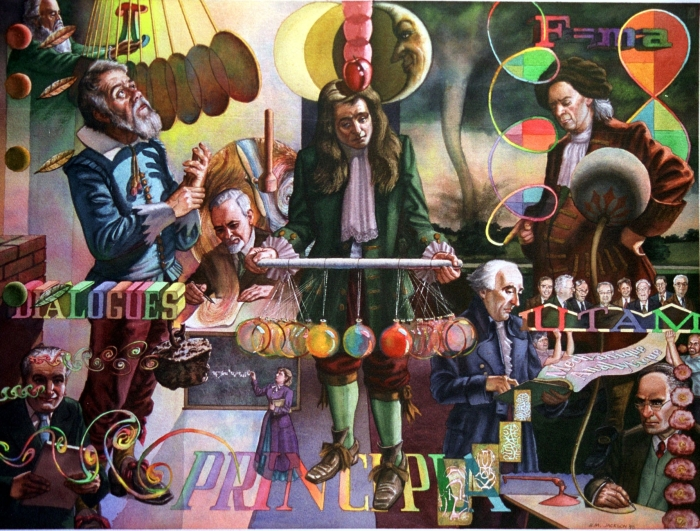
\includegraphics[width=.6\linewidth]{figures/template/Meters_of_Motion}
\caption{``Meter of motion'', adpated from \citep{jackson}.\label{fig:example}}
\end{figure}

If the figure occupies more than 70\% of the page area (leaving only 30\% for text) consider adding the figure alone in one page.

\subsection{Equations}

Equations are easily typed in \LaTeX. They are usually added within paragraphs, as part of the sentence. Please keep in mind that the sign $=$ could be considered a ``verb''. They also are number and may be referred, e.g.\ eq.~\ref{eq:ns}. An example is the Navier-Stokes equations stated for newtonian incompressible flows as
\begin{equation}
   \rho \left( \frac{\partial \boldsymbol{V}}{\partial t} + \boldsymbol{V}\cdot \nabla \boldsymbol{V} \right) = -\nabla p + \mu \nabla^2 \boldsymbol{V} + \rho \boldsymbol{g}. \label{eq:ns}
\end{equation}
Equations are centred on the page and it is recommended to enumerate all equations.



\subsection{References}

It is highly recommended to user BibTex file and style. Some examples of citations are in the following list 
\begin{itemize}
    \item \verb+\cite{einstein}+ \cite{einstein}
    \item  \verb+\citet{einstein}+ \citet{einstein}
    \item \verb+\citep{einstein}+ \citep{einstein}
\end{itemize}

By the end of the main .tex file there are the declaration of style \verb+Ref_Style.bst+, which should not be changed, and the list of .bib files, her\verb+RCGI.bib+ as an example.

% RANDOM TESTS
\blinddocument
	
	
	
% -----------------------------------------
% References
% -----------------------------------------
\bibliographystyle{Ref_Style} % style based in JFM
%\clearpage \phantomsection \addcontentsline{toc}{chapter}{References}
\bibliography{RCGI} % .bib archive with reference

% -----------------------------------------
%Appendix
% -----------------------------------------
\appendix
%\watermark{} % retirar a marca d'água

\chapter{Appendix I}

\section{Cras eget nulla enim}
Cras eget nulla enim. Sed vel neque vitae nibh ullamcorper euismod. Phasellus venenatis felis sem, sit amet accumsan magna ultrices quis. Vestibulum ullamcorper scelerisque augue commodo commodo. Cras commodo ante ac consequat placerat. Aliquam quis justo semper, molestie nulla sed, porta est. Aenean arcu metus, volutpat non lectus non, tincidunt varius felis. Interdum et malesuada fames ac ante ipsum primis in faucibus. Ut pretium neque quis leo faucibus, ac rutrum nisi dapibus. Vivamus nibh ex, semper et massa quis, porta rhoncus sapien. Nam euismod leo risus, vitae consequat ante pretium ac. Fusce fringilla cursus elit dapibus consectetur. Pellentesque vulputate tempus pulvinar. Sed arcu nisl, placerat eu ex nec, sagittis commodo nisi. Nam in mi eleifend, pharetra lacus sit amet, elementum arcu. Etiam arcu lorem, lacinia vel aliquam ac, venenatis auctor elit.

\section{Vestibulum eget quam neque}
Vestibulum eget quam neque. Suspendisse hendrerit tempus risus sed volutpat. Mauris vehicula luctus turpis nec pretium. Quisque sit amet finibus mauris, at dapibus orci. Nunc a accumsan turpis. Phasellus euismod nisi in turpis lacinia cursus. Vestibulum orci lectus, hendrerit ac lacinia vitae, viverra sit amet ipsum. Aenean congue sagittis nulla, non pharetra elit rutrum vitae. Praesent euismod justo vel orci luctus, vulputate bibendum ipsum congue. Praesent et nisl et massa aliquet viverra at et purus.

Nunc eu venenatis metus. Sed ac cursus ante. In mi ex, sollicitudin a dui in, vehicula posuere erat. Ut placerat commodo nisi sit amet auctor. Nam aliquam ante eu nulla commodo mollis. Aliquam ac ante quis dolor semper tempus. Donec pretium arcu sit amet dignissim gravida. Maecenas et ante eu lacus congue aliquam ac nec dolor. Aenean et rhoncus leo. Curabitur ullamcorper, mi ultricies ornare tempor, purus eros dapibus leo, vitae aliquet nibh elit vel felis. Nunc condimentum a nunc sed venenatis. Cras volutpat luctus purus, in rhoncus est placerat at. Vivamus sit amet turpis mi.

\chapter{Appendix II}

\section{Sed vel neque vitae nibh ullamcorper euismod.}
Cras eget nulla enim. Sed vel neque vitae nibh ullamcorper euismod. Phasellus venenatis felis sem, sit amet accumsan magna ultrices quis. Vestibulum ullamcorper scelerisque augue commodo commodo. Cras commodo ante ac consequat placerat. Aliquam quis justo semper, molestie nulla sed, porta est. Aenean arcu metus, volutpat non lectus non, tincidunt varius felis. Interdum et malesuada fames ac ante ipsum primis in faucibus. Ut pretium neque quis leo faucibus, ac rutrum nisi dapibus. Vivamus nibh ex, semper et massa quis, porta rhoncus sapien. Nam euismod leo risus, vitae consequat ante pretium ac. Fusce fringilla cursus elit dapibus consectetur. Pellentesque vulputate tempus pulvinar. Sed arcu nisl, placerat eu ex nec, sagittis commodo nisi. Nam in mi eleifend, pharetra lacus sit amet, elementum arcu. Etiam arcu lorem, lacinia vel aliquam ac, venenatis auctor elit.

\section{Mauris vehicula luctus turpis nec pretium}
Vestibulum eget quam neque. Suspendisse hendrerit tempus risus sed volutpat. Mauris vehicula luctus turpis nec pretium. Quisque sit amet finibus mauris, at dapibus orci. Nunc a accumsan turpis. Phasellus euismod nisi in turpis lacinia cursus. Vestibulum orci lectus, hendrerit ac lacinia vitae, viverra sit amet ipsum. Aenean congue sagittis nulla, non pharetra elit rutrum vitae. Praesent euismod justo vel orci luctus, vulputate bibendum ipsum congue. Praesent et nisl et massa aliquet viverra at et purus.

Nunc eu venenatis metus. Sed ac cursus ante. In mi ex, sollicitudin a dui in, vehicula posuere erat. Ut placerat commodo nisi sit amet auctor. Nam aliquam ante eu nulla commodo mollis. Aliquam ac ante quis dolor semper tempus. Donec pretium arcu sit amet dignissim gravida. Maecenas et ante eu lacus congue aliquam ac nec dolor. Aenean et rhoncus leo. Curabitur ullamcorper, mi ultricies ornare tempor, purus eros dapibus leo, vitae aliquet nibh elit vel felis. Nunc condimentum a nunc sed venenatis. Cras volutpat luctus purus, in rhoncus est placerat at. Vivamus sit amet turpis mi.

\end{document}
